En esta sección se detallarán los casos de uso y escenarios pertenecientes al subsistema de gestión de debates.
La figura \ref{fig:casos_uso_subsistema_debates} muestra el diagrama de casos de dicho subsistema.

\begin{figure}[h]
\centering
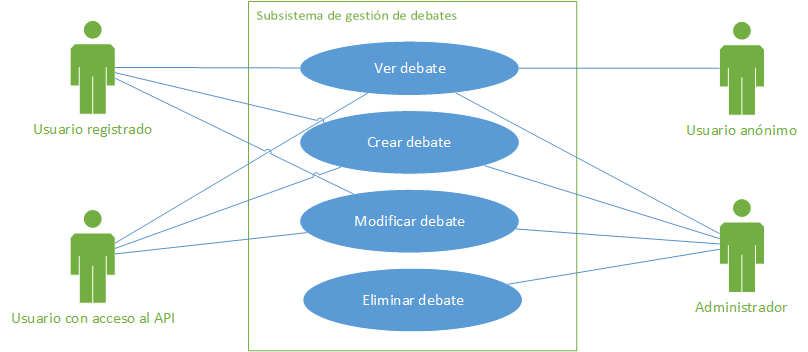
\includegraphics[width=\textwidth]{casos_uso_debates.png}
\caption{Diagrama de casos de uso del subsistema de gestión de debates}
\label{fig:casos_uso_subsistema_debates}
\end{figure}


\subsubsection{Caso de uso ``ver debate''}
\begin{description}
\item[Descripción] 				El usuario quiere ver el contenido y los comentarios de un debate.
\item[Actores] 					Cualquier rol de usuario registrado o no en el sistema.
\item[Escenario principal]	 	\hfill
								\begin{enumerate}
								\item El usuario accede a la vista de los debates.
								\item Una vez en la vista de debates, elige el debate del que quiere ver sus contenidos.
								\item El usuario pulsa en el título del debate elegido.
								\item El sistema carga la vista del debate mostrando tanto el contenido como los comentarios del mismo.
								\end{enumerate}
\end{description}


\subsubsection{Caso de uso ``crear debate''}
\begin{description}
\item[Descripción] El usuario quiere crear un nuevo debate para que puedan participar el resto de usuarios.
\item[Actores] Administrador, usuario registrado o usuario con capacidad de acceso al API.
\item[Precondiciones] Haber iniciado sesión en el sistema.
\item[Escenario principal] \hfill
						 	\begin{enumerate}
							\item El usuario accede a la vista de debates.
							\item Pulsa el botón para crear un debate.
							\item Rellena los campos requeridos en el formulario de creación del debate.
							\item Rellena los campos opcionales que considere necesarios en el formulario de creación del debate.
							\item Pulsa el botón para guardar el debate.
							\item El sistema guarda el debate con estado \textit{próximamente}.
							\end{enumerate}
\item[Escenario alternativo 1] El usuario no ha rellenado todos los campos requeridos.
							\begin{enumerate}
							\item El sistema notificará al usuario de que faltan campos por rellenar.
							\item Se continuará desde el punto 3 del escenario principal.
							\end{enumerate}
\end{description}


\subsubsection{Caso de uso ``modificar debate''}
\begin{description}
\item[Descripción] Un usuario quiere modificar el contenido de un debate.
\item[Actores] Administrador, usuario registrado o usuario con capacidad de acceso al API.
\item[Precondiciones] Haber iniciado sesión en el sistema.
\item[Escenario principal] \hfill
						 	\begin{enumerate}
							\item El usuario accede a la vista de debates.
							\item Selecciona el debate cuyo contenido desea modificar.
							\item Una vez en el debate adecuado, pulsa el botón destinado a modificarlo.
							\item Modifica la información que sea necesaria (excepto el estado del debate, el proceso de modificación del estado de un debate está descrito en el escenario alternativo 1).
							\item Pulsa el botón para guardar las modificaciones.
							\item El sistema guarda los cambios y actualiza los contenidos del debate.
							\end{enumerate}
\item[Escenario alternativo 1]  Modificar el estado de un debate.
							\begin{enumerate}
							\item El administrador accede al panel de administración.
							\item Selecciona el debate que desea modificar y pulsa el botón correspondiente.
							\item En la vista de edición del debate selecciona el nuevo estado que desea asignarle.
							\item Se continúa desde el punto 5 del escenario principal.
							\end{enumerate}
\item[Escenario alternativo 2]  No se rellenan todos los campos requeridos
							\begin{enumerate}
							\item El sistema informa al usuario del error y no modifica la información almacenada.
							\item Se continúa desde el punto 4 del escenario principal.
							\end{enumerate}
\end{description}


\subsubsection{Caso de uso ``eliminar debate''}
\begin{description}
\item[Descripción] El administrador quiere eliminar un debate.
\item[Actores] El administrador del sistema.
\item[Precondiciones] Haber iniciado sesión en el sistema.
\item[Escenario principal] \hfill
						 	\begin{enumerate}
							\item El administrador accede a la vista de administración.
							\item Localiza el debate que desea eliminar y pulsa el botón correspondiente.
							\item El debate será eliminado del sistema.
							\end{enumerate}
\end{description}